\chapter{Experimental}
\label{chap4}

\section{Methodology}
\label{sec:method}

Because the work in this project is based on the pre-existing code found in the CV32E40S repository\cite{cv32e40s_manual}, some design considerations had to be made when implementing the dual core. For instance, removing features from the Xsecure ISE is easier said than done due to the features being heavily woven into many aspects of the core and the verification environment. Because of this, it was decided that only removing the PCH feature would be a good baseline for testing and comparison between the old and new architectures. This means that the two architectures being compared are: \textbf{The unmodified CV32E40S core} and \textbf{The modified Dual-Core Lockstep CV32E40S with PCH removed}. To test that the architectures work they both run a \textit{sanity} simulation of the code shown in \autoref{app:helloworldC} using \textit{Verilator}\cite{verilator}.

Direct comparison between the cores is done by looking at the number of clock cycles needed to run through the test program, as well as the area and power usage of the synthesized design. These comparisons are done mostly to give some understating of the resource usage, but for evaluating the effectiveness of the solution these metrics are not very useful. As these cores are both meant to be used in applications where hardware security is of the utmost importance, they are often allowed to trade PPA for robustness. Because of this, both cores will be tested against a simple program, shown in \autoref{lst:test_code}, representing a secure boot protocol similar to the one shown in \autoref{fig:glitchable_code}. The idea behind the test is to simulate a glitch attack happening at different places in the execution of the program and to see how both architectures will handle it. Because we only removed the PCH feature, the glitching will be restricted to the PC. This means we will only try to do instruction skipping, and no resetting of register values or status registers for conditional branches. 

\subsection{Skipping instructions}
\label{subsec:skip_instr}

In a practical system, manipulating the program counter to specific values can be challenging. However, utilizing voltage- or clock-glitching techniques allows for the disruption of the normal logic behavior responsible for incrementing the program counter. This interference enables the incrementation of the pointer multiple times, effectively skipping one or more instructions. Consequently, if an attacker possesses knowledge of the execution sequence, they can strategically skip branches or jumps, gaining unauthorized access to restricted sections of the code.

In cases where the attacker has limited insight into the instruction sequence but has access to the system's bootloader, an alternative method for instruction skipping exists. By inserting numerous 'NOP' instructions before the targeted restricted code area, the attacker can 'scramble' the program counter, and have an increased likelyhood of landing on a 'NOP'. From this instruction the system continues sequential execution, eventually reaching the desired restricted code.

\section{Simulating instruction skipping}
\label{sec:sim_instr_skip}

Because the tests are restricted to instruction skipping, it limits the potential ways suck a simple program can be exploited. However, the tests shown in \autoref{tab:instr_skip_test} will be run on the code shown in \autoref{lst:test_code}. Most, if not all, of the code in the test is somewhat redundant. Because of this, the code is compiled with the '-O0' flag. This way, the C-code and RISC-V assembly are as closely related as possible. The assembly for the test program is shown in \autoref{lst:asm_instr_skip}. 

\begin{lstlisting}[caption={A sample C++ code}, label=lst:test_code, language=C++]
int main(int argc, char *argv[])
{
    int result_code = 0;

    /* Count to avoid actual infite loop */
    unsigned int count = 0;

    /* Get error result code */
    result_code = boot_go();

    if (result_code != 0) {
      while(1) {
       	if (count > 10)	{
          printf("Exiting...\n");
       	  return EXIT_SUCCESS;
        }
        count++;
      }
    }

    printf("Glitched out of loop\n");
    do_boot();
    return EXIT_FAILURE;
}
\end{lstlisting}

\begin{table}[h]
\centering
\caption{Instruction skipping tests.}
\label{tab:instr_skip_test}
\begin{tabular}{m{2.5cm}m{3.5cm}m{7.5cm}}
\toprule 
Line in C code & ASM instruction & Expected outcome \\
\midrule
\rowcolor{black!20} \textbf{11} & sw x10,-24(x8) & Skipping this instruction means that the value of '-1' from the 'boot\_go()' function is never stored in the 'result\_code' register. The program then never enters the scope of the conditional statement. \\
\textbf{15} & c.j 458 $\langle$main+0x20$\rangle$ & Skipping the jump instruction that keeps the 'while(1)' loop repeating will glitch out of the scope of the loop and execute the 'do\_boot()' function.  \\
\rowcolor{black!20} \textbf{Any line} & Any instruction & From any point in the code it is potentially possible to glitch directly to the address of the 'do\_boot()' function. The real danger of this happening is discussed in \autoref{subsec:skip_instr}. \\
\bottomrule
\end{tabular}
\end{table}

\section{Coverage tests}
\label{sec:coverage_test}

While it is important to check whether the Dual-Core setup can replace some of the specific security features of \textit{Xsecure}, it does not explore one of the main advantages: glitch detection coverage. In order to test coverage, we will introduce glitches in areas that are not specifically covered by \textit{Xsecure}. One such area is the address-bus going to the data-memory during a load or store instruction. If this were to happen with only one core, the wrong data might stay in the memory undetected and faults can propagate to other parts of the execution sequence. With Dual-Cores any discrepancy between the loaded or stored data can be detected before faults distrupt the system. 

Other glitches that are not covered by \textit{Xsecure} are glitches affecting the \textit{a} or \textit{b} operands 

\textbf{Teste om jeg rekker: Glitche adressebussen fra en load/store instruksjon. Glitche operand a eller b når den er i id stage. I execute må man glitch a eller b i id\_ex\_stage}

\subsection{How are the different layouts tested?}
\subsubsection{Synthesis tool - Which one is used?}
\subsubsection{How is fault injection done in sumlation?}
\subsection{How are results from fault injection compared between the different setups?}

\section{Dual RISC-V Cores in lockstep}
\label{sec:dualcore}

The proposed dual-core architecture is quite straight forward to implement. All that is needed is to connect two cores with synchronization registers at appropriate intervals. Choosing the correct granularity for comparisons is however important. At the highest level, comparing only the output of both cores is an option. Comparison would then have to be done in the \textit{write-back} stage of the pipeline. For the end-user application, this would be the most natural way to do it as the details of what has glitched is far less important than just detecting an error. However, for analyzing the effects of glitch attacks on a system in more detail, a much more fine grained approach is needed. The obvious counterpart to only comparing the output would be to compare all wires and registers. This would allow the user to determine the exact location of an error, but at the cost of adding a lot of hardware. This way of implementing the comparisons can also be argued against as it goes against one of the principal ideas of using a dual-core lockstep mechanism: simplicity of integration. 

As the purpose of this project is to analyze the effectiveness of the dual-core lockstep mechanism, some granularity is needed. However, knowing exactly which wire or register bit has glitched will not be necessary, and adds a lot of extra work for simply connecting everything. Therefore, synchronization registers where comparison happens will be connected to the input signals going to different stages of the pipeline. From this data it is then possible to detect a glitch and give the user some information about exactly where in the pipeline the fault occurred. The top level block diagram for the dual-core lockstep setup is seen in \autoref{fig:dual_block}. As an added security measure, the two cores should be intentionally offset from each other by a few clock cycles. This way, in the unlikely event that an attacker manages to glitch the two cores in precisely the same way at the same time, they now need to do it in a highly synchronized manner, which significantly increases the complexity of the attack. The deliberate offset between the cores introduces a form of time diversity, making it more challenging for an attacker to exploit vulnerabilities using clock glitches or other timing-based attacks. These additional security measures enhance the system's resistance to fault injection attacks and improve its overall robustness.

\begin{figure}[h!]
    \centering
    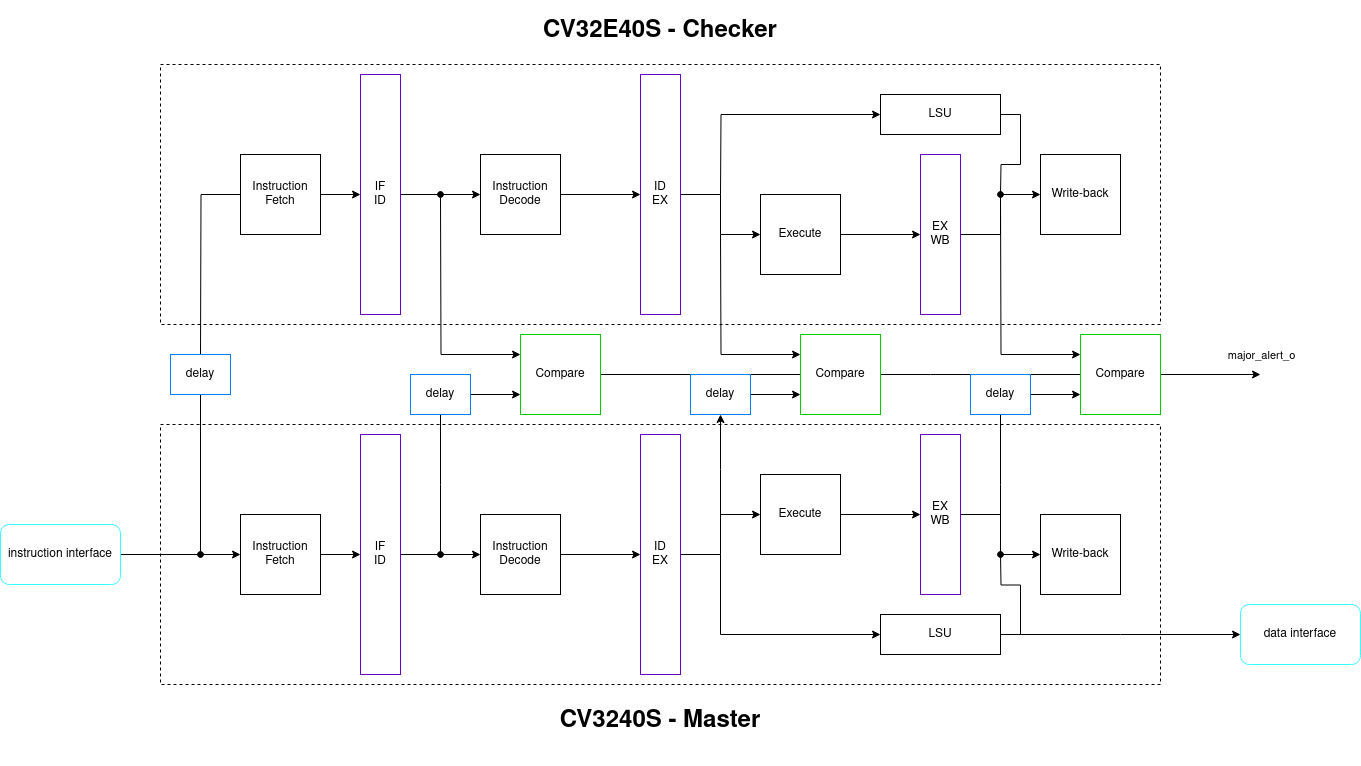
\includegraphics[width=\textwidth]{docs/images/dual_cores_block.png}
    \caption{Block diagram cv32e40s dual-core lockstep mechanism.}
    \label{fig:dual_block}
\end{figure}

\textbf{Instruction to be glitched:}
\begin{lstlisting}
       30003.000 ns | 0000672c | memchr syscalls.c 379 - beq x14,x10,66b4 <memchr+0x3c>
\end{lstlisting}

In order to glitch the loop we need to make the program skip the instruction that happens at 29991.000 ns. This is a bne instruction that keeps us in the loop. Next instruction occurs at 29997 and we must therefore chang ethe program counter before this. 

Glitch 6734 to 673c

Count lagret i x8 
Verdien 10 lagret i x9

\section{Limitations}
\label{sec:limit}

\section{Choices / Findings}
\label{sec:choice}